\section{Umsetzung des Self-Service}
Zur Umsetzung des Self-Service wurde das Framework~\textit{Angular 9}~\cite{angular} verwendet. Der gesamte Quellcode ist im GitHub-Repository \textit{MariamaB/tbc-app}~\cite{github_tbc} verfügbar. Mithilfe der~\textit{\textbf{N}ode \textbf{P}ackage \textbf{M}anager}~\cite{npm} (npm) und der Angular CLI wurde ein Angular Projekt aufgesetzt und alle weiteren packages installiert. Zudem wurden Hauptsächlich die Komponenten der ~\textit{Angular Material}~\cite{angularmaterial} Library verwendet um die UI zu entwickeln. Neben weiteren packages wurde~\textit{JsPDF}~\cite{jspdf} zur Generierung und Bereitstellung der PDF download Funktion eingesetzt.
\\\\
Die Nutzeroberfläche hat derzeit zwei Zustände. Im 1. Zustand hat der Nutzer die Möglichkeit die gefragten Informationen direkt ins Canvas einzugeben Abbildung~\ref{fig:canvasonedit}. Diese hätte auch mit einen Fragebogen gelöst werden können, jedoch bekommt der Nutzer so einen besseren Überblickt was noch gefragt ist und kann sich quasi die Reihenfolge der Bearbeitung nach belieben aussuchen. Außerdem kann so am Ende alles auf einem Blick gegen geprüft werden und bei Unzufriedenheit oder Unvollständigkeit nach gebessert werden.
\begin{figure}[H]
	\centering
	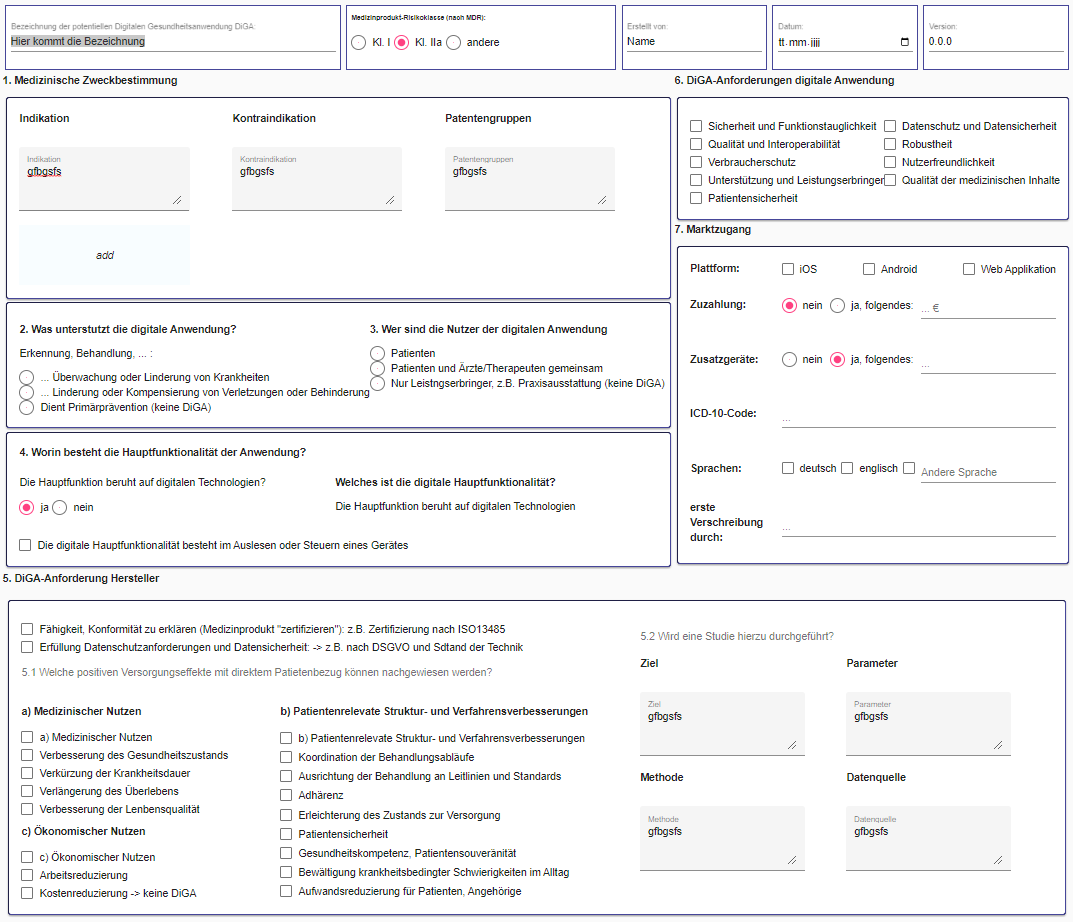
\includegraphics[width=350px, keepaspectratio]{assets/onEdit.png}
	\caption[DiGA-Canvas - Bearbeitungsmodus]{DiGA-Canvas - Bearbeitungsmodus,~Quelle: Eigene Entwicklung}
	\label{fig:canvasonedit}
\end{figure}
Der 2. Zustand ist die gespeicherte Version des Canvas Abbildung~\ref{fig:canvasonsave}. Zu diesem Status kommen zwei weitere Felder:
\begin{itemize}
	\item Welches sind die nächsten Schritte des Herstellers?
	\item Gebühren und Auslagen für Hersteller
\end{itemize}
 Das sind Felder, die von dem Self-Service zur Information des Herstellers nach Bearbeitung des Canvas ausgewertet und befüllt werden. Anschließend besteht die Option diesen Canvas in dieser Form als PDF zu downloaden.
  \begin{figure}[H]
  	\centering
  	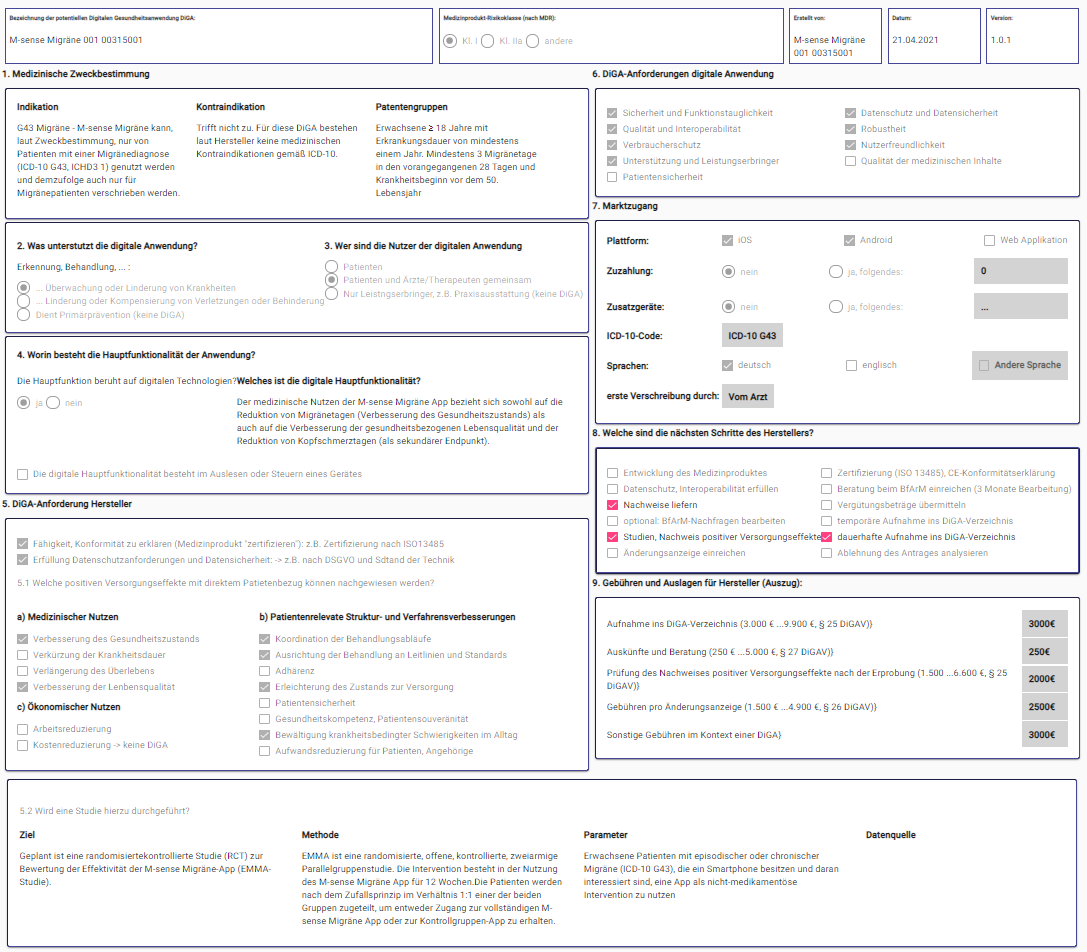
\includegraphics[width=350px, keepaspectratio]{assets/onSave.png}
  	\caption[DiGA-Canvas - Gespeicherter Modus]{DiGA-Canvas - Gespeicherter Modus,~Quelle: Eigene Entwicklung}
  	\label{fig:canvasonsave}
  \end{figure}
Als Background Komponente wird eine~\textit{Firebase}~\cite{firebase} Realtime Datenbank verwendet. In der alle eingegebenen und generierten Daten verwaltet werden. Mittels der~\textit{Angularfire}~\cite{angularfire} Library interagiert das Angular Projekt direkt mit der Firebase Datenbank. Über die Firebase Console lassen sich die Daten verwalten und einsehen.
  
    \begin{figure}[H]
  	\centering
  	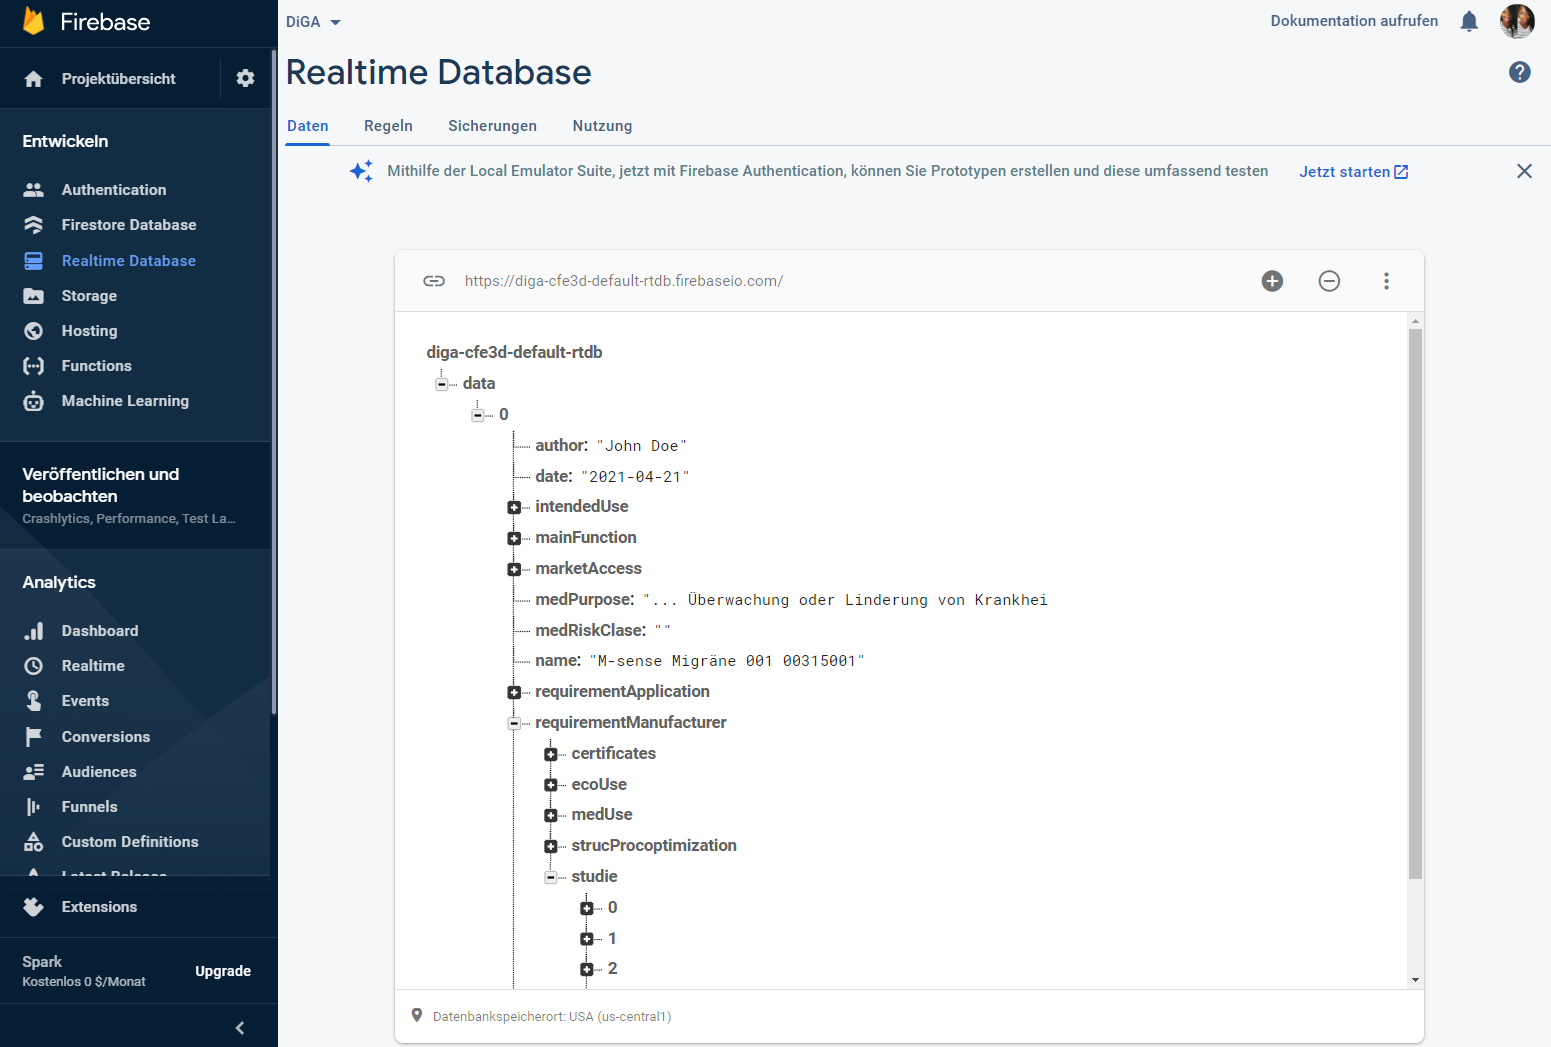
\includegraphics[width=350px, keepaspectratio]{assets/firebaseConsole.png}
  	\caption[Firebase Console - Realtime Database]{Firebase Console - Realtime Database,~Quelle:~\cite{firebase}}
  \end{figure}